\chapter{Detalles de implementación}\label{cap:implementation_details}

Con el objetivo de garantizar que el lector esté más acorde con la tecnología usada para la implementación, las razones de esa elección, la forma de desplegar el sistema y demás aspectos relacionados con la parte tecnológica se expone esta capítulo.

A día de hoy se cuenta con muchas herramientas para desarrollar un software de este tipo. En esta ocasión se escogión una tecnología que ha alcanzado bastante auge en los últimos años. En las secciones siguientes se hará alusión a la misma así como al lenguaje empleado para el desarrollo.

\subsection{Lenguaje de programación}
Para este proyecto se utilizó el lenguaje TypeScript, auxiliándonos de NestJS (framework de NodeJS).

\subsubsection{TypeScript}\cite{wiki_ts}

TypeScript es un lenguaje de programación libre y de código abierto desarrollado y mantenido por Microsoft. Es un superconjunto de JavaScript, que esencialmente añade tipos estáticos y objetos basados en clases. Anders Hejlsberg, diseñador de C\# y creador de Delphi y Turbo Pascal, ha trabajado en el desarrollo de TypeScript. TypeScript es usado para desarrollar aplicaciones JavaScript que se ejecutarán en el lado del cliente o del servidor, o extensiones para programas (Node.js y Deno).

TypeScript extiende la sintáxis de JavaScript, por tanto cualquier código JavaScript existente debería  funcionar sin problemas. Está pensado para grandes proyectos, los cuáles a través de un compilador de TypeScript se traducen a código JavaScript original. 

TypeScript soporta ficheros de definición que contengan información sobre los tipos de librerías JavaScript existentes; esto permite a otros programas usar los valores definidos en los ficheros como si fueran entidades TypeScript de tipado estático. El compilador de TypeScript está escrito asimismo en TypeScript. 


El lenguaje fue publicado en octubre de 2012 , después de dos años de desarrollo por parte de la compañía y desde esa fecha ha tenido en general, buena aceptación por parte de todos lo que le mereció el mérito en 2020 como segundo lenguaje de programción más amado según la encuesta de Stack Overflow\cite{stack_overflow} 2020 Develop Survey.

\subsubsection{NestJS}\cite{nestjs_doc}
NestJS es un framework para construir eficientes y escalables aplicación del lado del servidor utilizando NodeJS. Posee soporte tanto para JavaScript como para TypeScript y combina elementos de Programación Orientada a Objetos (OOP, por sus siglas en inglés), Programación Funcional y Programación Funcional Reactiva. 

Nest posee un robusto framework HTTP basado en \textit{Express} (definido por defecto) y opcionalmente se puede configurar además el uso \textit{Fastify} como alternativa a \textit{Express}.

Nest ofrece un nivel de abstracción superior al que normalmente encontramos en los demás frameworks de Node(Express/Fastify), pero también expone sus APIs directamente al desarrollador. Esto le ofrece a los desarrolladores la libertad de emplear la mayoría de las aplicaciones de 3ros desarrolladas para esos otros frameworks.

En los últimos años gracias a Node, JavaScript se ha convertido en una gran herramienta web tanto para front como para aplicaciones de backend. Se presentan impresionantes proyectos como Angular, React, Vue; los cuáles mejoran la productividad de los desarrolladores y hacen que el desarrollo de nuevos productos sea más rápido, más testeable y más extensible. Por otra parte y a pesar de las bondades que ofrece Node, aún no presenta una solución efectiva al problema de arquitectura. 

Nest se presenta como solución a esto, ya que posee una estructura que induce desde el principio a la utilización de patrones arquitectónicos. La arquitectura de Nest es inspirada en Angular.

Fue desarrollado por Kamil Mysliwiec, desarrollador de Google; el lanzamiento de su versión 9 se realizó el 8 de Julio de 2022.

\subsection{Aplicación visual}

La idea detrás de la aplicación visual surge inspirada en un sistema desarrollado hace un par de años dentro de la facultad por un grupo de estudiantes y que se presentó como proyecto a la jornada científica de ese curso. 

Se ofrece un sistema desarrollado en VueJS y que pretende seguir las buenas prácticas de desarrollo de frontend. Está escrito en JavaScript.

El sistema posee un conjunto de vistas dedicadas a manejar todas las tareas administrativas referentes al software; dígase: creación de profesores, grupos, semestres, asignaturas y demás cuestiones referentes al centro educacional. 

Solamente para el usuario con los permisos adecuados están habilitadas tales características, es decir el usuario administrador es el único que puede realizar modificaciones internas dentro del sistema.

En la página principal se definen 5 tipos de filtros que hacen posible una rápida interacción con el sistema. Estos filtros se presentan útiles en un gran número de escenarios. En la página principal se muestra además la opción de descargar el horario, esta está habilitada para cualquier tipo de usuarios. El número que se presenta en la parte superior izquierda es referente a la felicidad del sistema, aspecto que fue abordado en las secciones previas a este capítulo. (\ref{sec:happiness})

En la visualización general del horario, cada grupo posee un color específico para que se haga más sencilla su lectura, el color es posible definirlo por el administrador del sistema a la hora de la creación del grupo, luego todos los turnos de clase que se asocien al mismo, se mostrarán de ese color.

En el manejo de la interfaz visual quizá resulte un poco llamativo para el administrador del sistema; que es el que tiene acceso a esas vistas; la creación, modificación y eliminación en serie que se muestra en cada \textit{modal} referente a los turnos de clases.  Este aspecto fue abordado con anterioridad, pero la acción que realiza es modificar todos los turnos que posean las mismas características del turno actual, es decir, que repitan el ciclo del horario para él. Un ejemplo de esto se evidencia claramente en: todos los turnos del martes a 4to turno de Matemática Discreta para 2$^{do}$ de Ciencias de la Computación.

Para cada turno visualizado es valido además modificarle la duración del mismo, esto se logra modificando el \textit{size} de este dentro del horario. Realizar esta acción es justo como modificarle el \textit{size} a cualquier otra ventana del sistema, lo que en esta ocasión es al caja que describe el turno.

Haciendo clic encima del turno se obtine además una descripción detallada del mismo, así como las opciones para la edición múltiple.

\subsection{Autenticación}

La autenticación es una parte esencial en la mayoría de los sistemas y aplicaciones. Existe muchos formas y estrategias de manejar la misma. La autenticación dentro del sistema se maneja con un módulo independiente que posee todos los casos de uso y middlewares relacionados con tal aspecto. En esta ocasión el proceso se realiza por medio de JSON Web Token(JWT).

JWT es un estándar de internet propuesto para la creación de firmas y/o encriptación (opcional) cuyo contenido es enviado en forma de cadena de texto de backend a frontend (y viceversa). Los tokens que se generan son firmados usando un protocolo de clave pública y clave privada. La forma de funcionamiento de JWT resalta por su simpleza, el servidor se encarga de generar un token que puede contener información referente al usuario autenticado (en la mayoría de los casos maneja los permisos de los usuario, así como el ID). Este token es enviado del servidor al cliente y este último se encarga de almacenarlo en las cookies o el local storage. Luego el cliente en cada una de las peticiones adjunta este token y de esa forma el servidor puede identificar correctamente al usuario que pretende acceder a los puntos de acceso definidos.\cite{jwt_wiki}

Cuando se recibe una petición de login por parte del cliente, el servidor se encarga de comprobar que las credenciales son correctas y la respuesta del login, es entre otras cosas, el token al que se hace referencia en el párrafo anterior. Supongamos después que se hace otra petición cliente-servidor y que el token se adjunta de forma apropiada en las cabeceras de la misma, cuando la petición arriba al punto adecuado, el servidor se encarga de ejecutar un \textit{middleware} (función intermedia) que procesa el token y verifica que sea el correcto, si todo este proceso se ejecuta sin mayores contratiempos, entonces en el request de la petición a través del campo user (request.user) se puede acceder al usuario que está intentado realizar la acción. En otro caso se responde con un estado 401 lo que indica que el usuario no esta autorizado al acceder al recurso que intenta solicitar. 

Todo este proceso antes descrito se realiza por medio de un paquete de terceros \textit{@nestjs/jwt} y además con la intervención de \textit{passport-jwt}

\begin{figure}[h!]
	\centering
	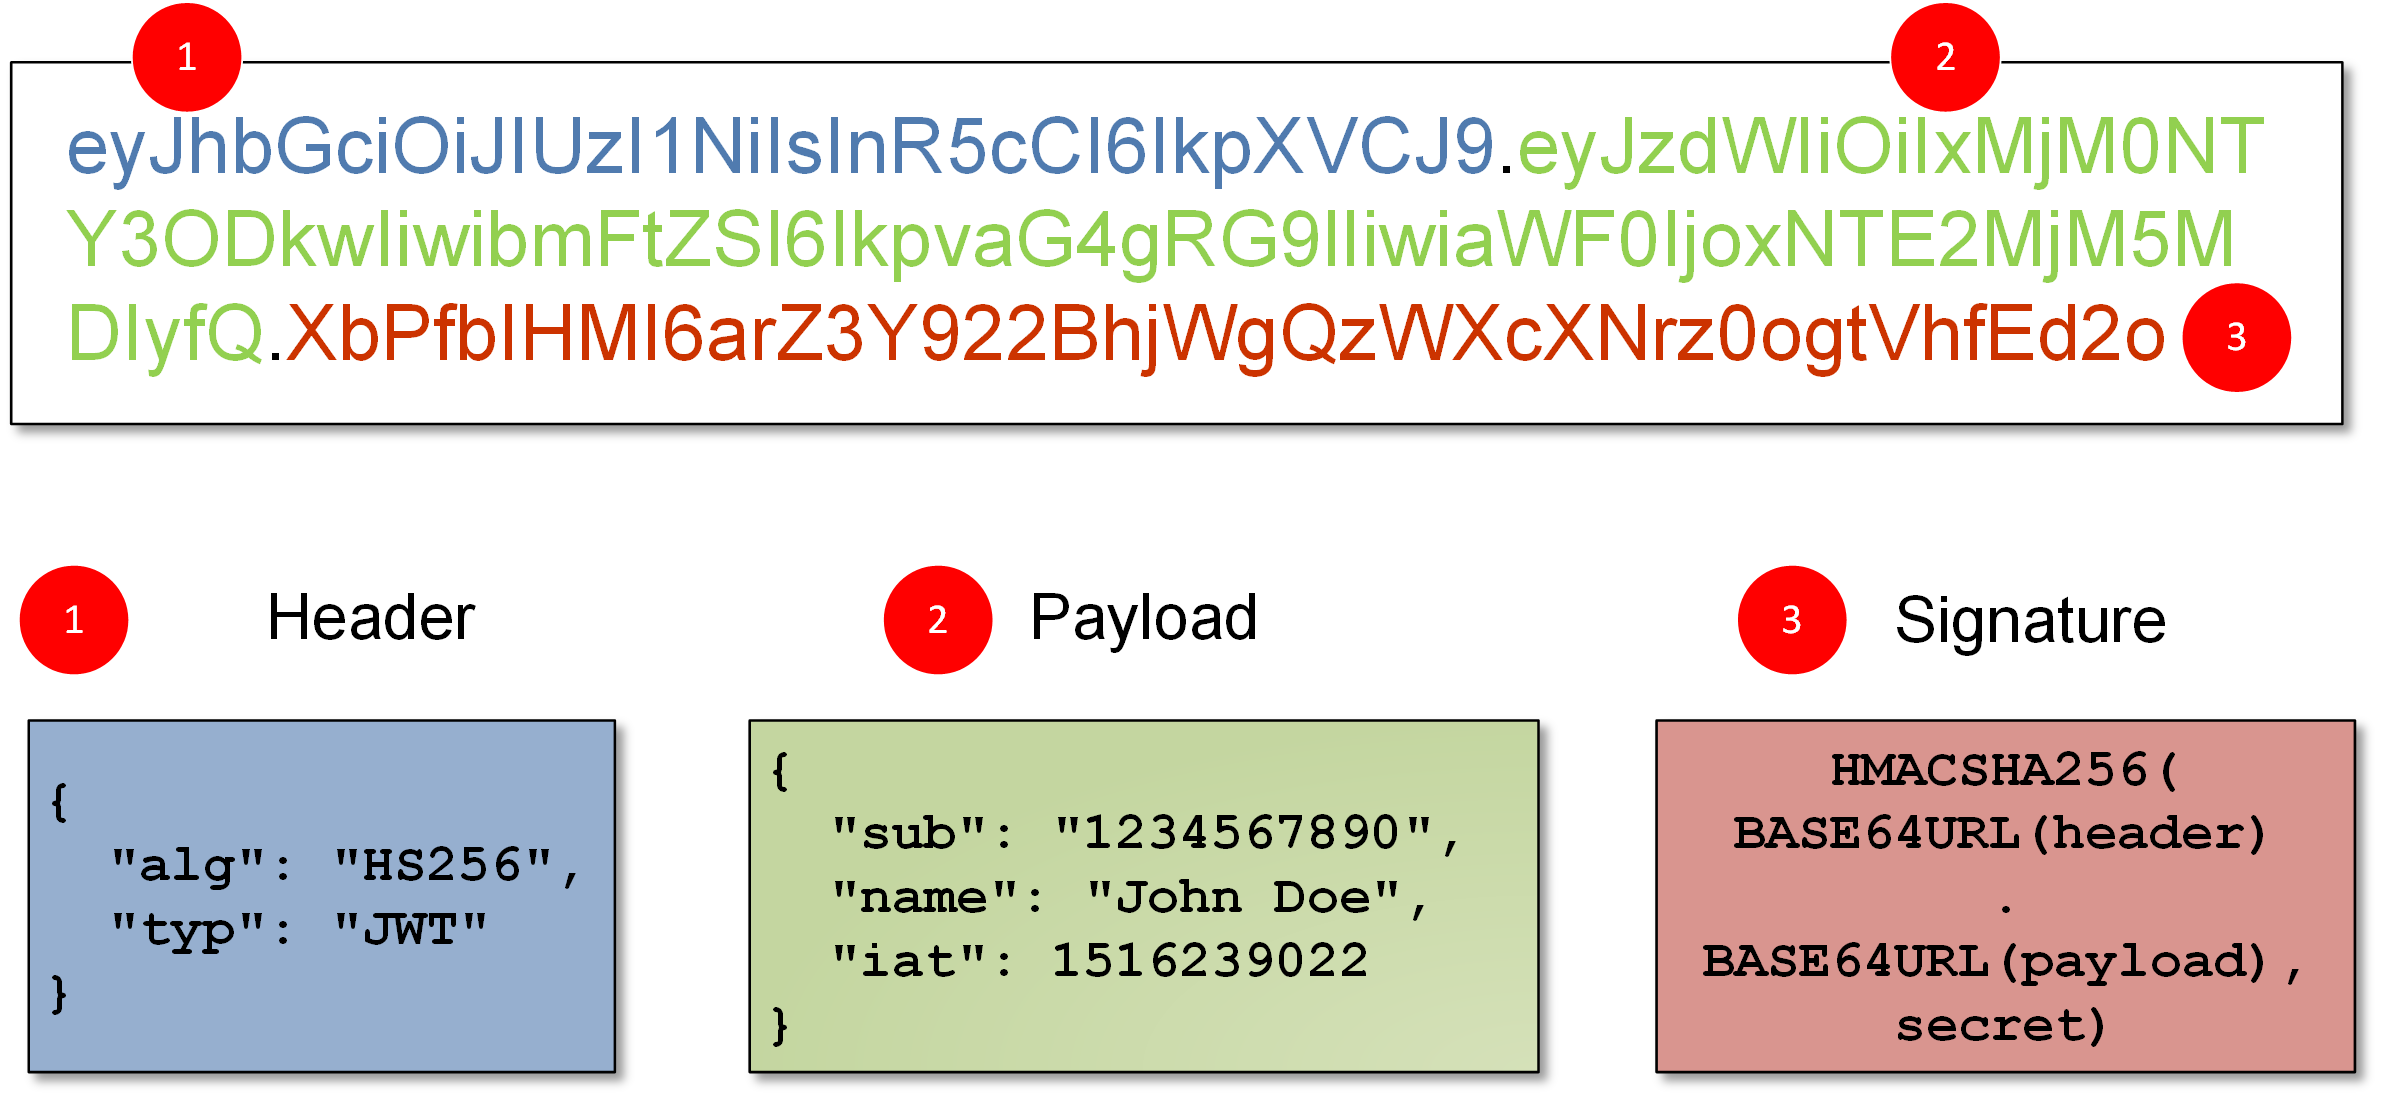
\includegraphics[width=0.95\linewidth]{images/Chapter 2/jwt1}
	\caption{Estructura del token}
	\label{fig:jwt}
\end{figure}

\subsection{Roles y Usuarios}







